\section{Inversión de Sistemas}
	Sea
	\begin{align}
		y = S_{a}(x) \\
		y[n] = \frac{1}{2}y[n-1]-x[n]
		\label{eq:considerations_system_inversion}
	\end{align}
	\subsection{Encontrar el sistema inverso}
		Buscamos obtener
		\begin{align}
			\delta[n] = S_{b}(S_{a}(\delta[n]))
			\label{eq:system_inverse_target}
		\end{align}
		
		Para encontrar el sistema $S_{b}$ que satisface lo anterior, es conveniente expresar la ecuación \ref{eq:considerations_system_inversion}, mediante su función de transferencia, aplicamos transformada Zeta:
		\begin{align}
			Y[z] = \frac{1}{2}Y[z]Z^{-1} - X[z] \\
			Y[z] \left( 1 - \frac{1}{2}Z^{-1} \right) = -X[z] \\
			H_{a}[z] = \frac{Y[z]}{X[z]} = \frac{2Z}{1 - 2Z}
			\label{eq:transfer_function_ha}
		\end{align}
		

		Con esta función de transferencia, buscamos que al aplicar ambos sistemas a una señal de entrada, el resultado sea la misma señal de entrada, esto equivale a poner ambos a poner ambos sistemas en cascada:
		\begin{equation}
			S_{b}(S_{a}(x[n])) \equiv h_{b}[n] * h_{a}[n] * x[n] = x[n]
		\end{equation}
		
		En términos de la transformada Zeta:
		\begin{equation}
			H_{a}[z] \cdot H_{b}[z] \cdot X[z] = X[z] \Longleftrightarrow H_{a}[z] \cdot H_{b}[z] = 1
 		\end{equation}
 		
 		Por lo que podemos definir:
 		\begin{equation}
 			\boxed{H_{b}[z] = \frac{1}{H_{a}[z]} = \frac{1 -2Z}{2Z}}
 		\end{equation}
 		
 		De esta forma, encontramos la respuesta a impulso que debe tener el sistema inverso, volviendo a ecuaciones en diferencia, expresamos el sistema:
 		\begin{equation}
 			\boxed{y[n] = -x[n] + \frac{1}{2}x[n-1]}
 			\label{eq:2_inverse_system}
 		\end{equation}
 		
 	\subsection{Implementación en Matlab}
 		Implementando ambos sistemas como funciones en Matlab:
 		
 		\begin{figure}[H]
 			\lstinputlisting[language=Matlab, firstline=49, lastline=61]{../parte_ii.m}
 		\end{figure}
 		
 		\subsubsection{Respuesta a impulso de Sa(x)}
 			\begin{figure}[H]
 				\center
 				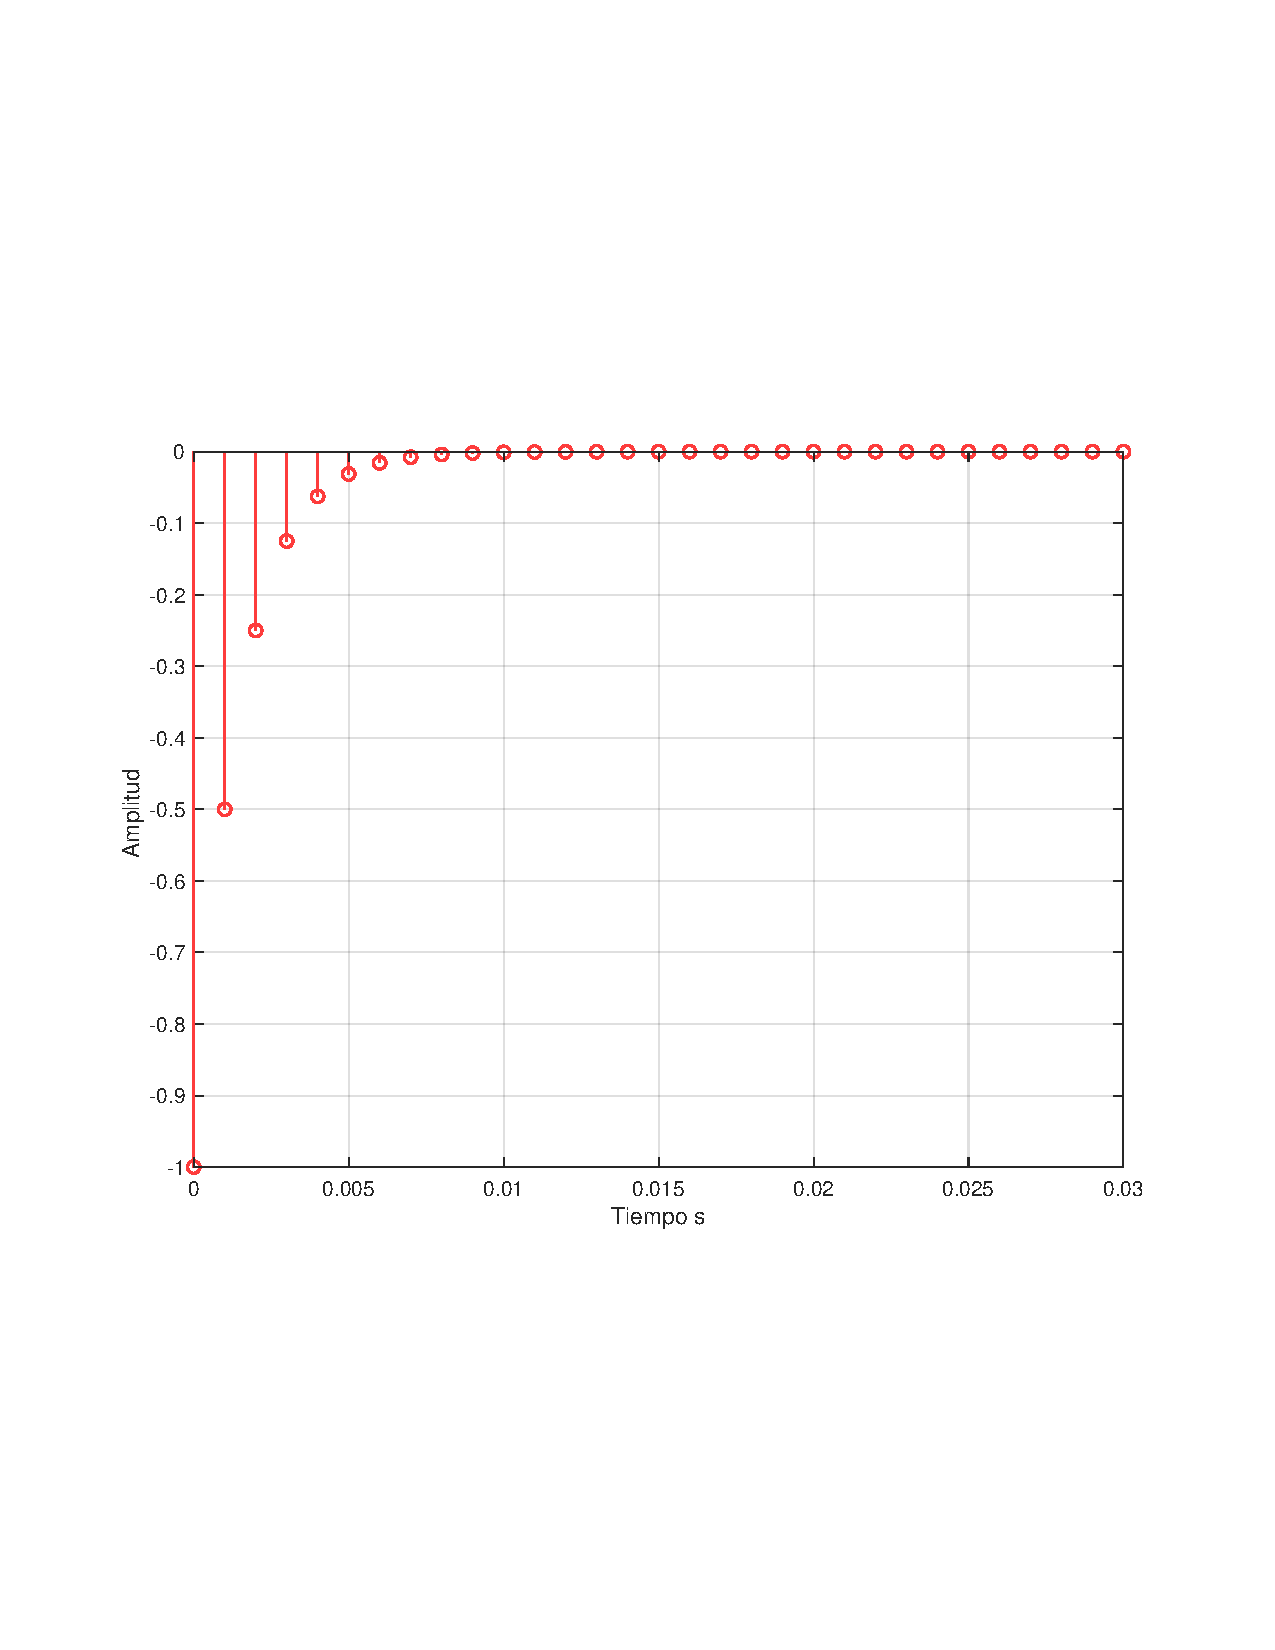
\includegraphics[width=0.6\textwidth,clip, trim = {2cm 7.0cm 2.2cm 7.0cm}]{../imgs/2_Sa.pdf}
				\caption{Respuesta del sistema $S_{a}(x)$ a impulso}
 				\label{fig:2_Sa}
 			\end{figure}
			Analizando la respuesta de este sistema, podemos comprobar lo descrito en la ecuación \ref{eq:considerations_system_inversion}, el valor actual de la salida, corresponde a 0.5 el valor anterior de la salida, menos el valor actual. Como el delta solo se aplica en t = 0, la salida parte con un valor negativo y se va reduciendo por un factor de 0.5 a medida que avanza el tiempo. 
			
 		\subsubsection{Respuesta a impulso de Sb(x)}
 			\begin{figure}[H]
 				\center
 				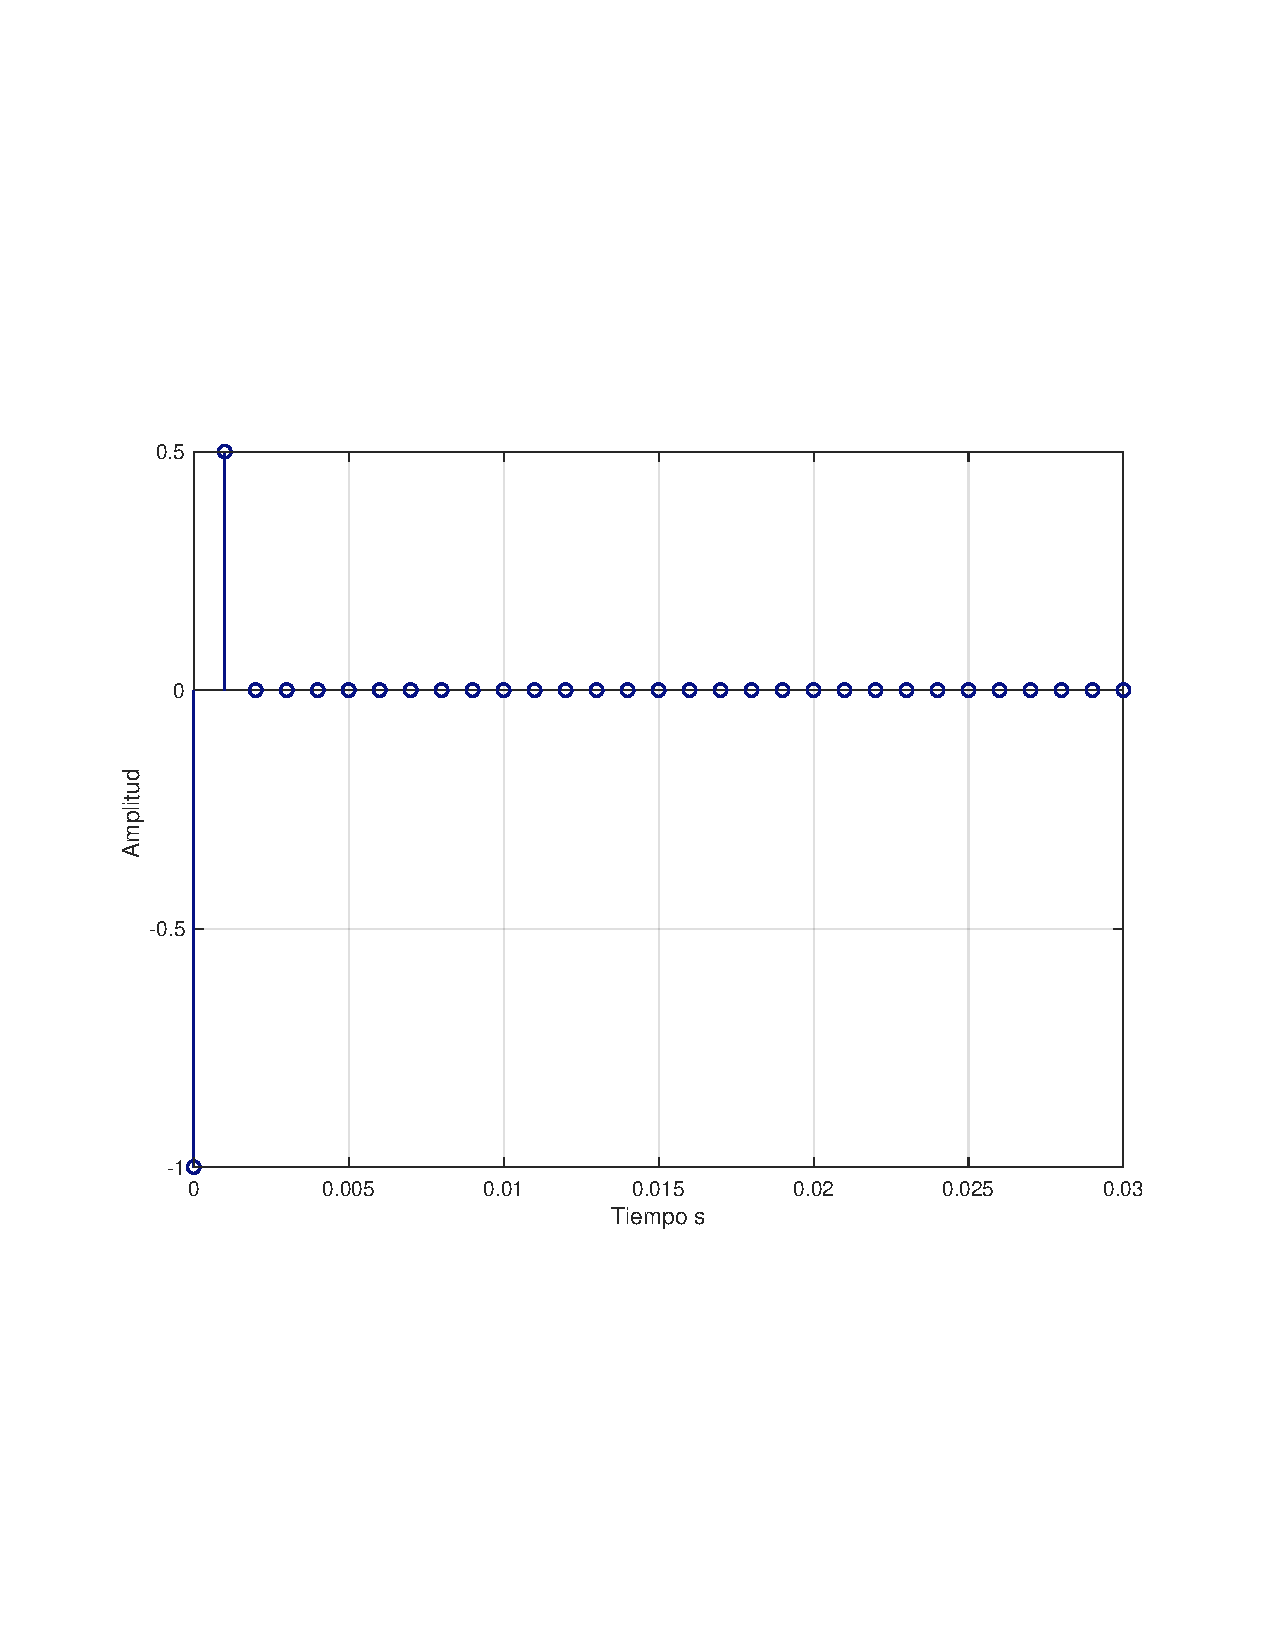
\includegraphics[width=0.6\textwidth,clip, trim = {2cm 7.0cm 2.2cm 7.0cm}]{../imgs/2_Sb.pdf}
				\caption{Respuesta del sistema $S_{b}(x)$ a impulso}
 				\label{fig:2_Sb}
 			\end{figure}
 			
 			Comparando el resultado con lo esperado con la ecuación \ref{eq:2_inverse_system}, notamos que el sistema toma el valor actual de la salida, escalado por -1 y 0.5 veces el valor anterior de la entrada, es por esto que con un delta en t = 0  como entrada,  la salida primero se dispara a -1 (la señal anterior a t = 0 es 0), para al siguiente instante, tomar valor 0.5 y al siguiente mantenerse en cero. 
		\subsubsection{Respuesta a impulso de Sb(Sa(x))}
 			\begin{figure}[H]
 				\center
 				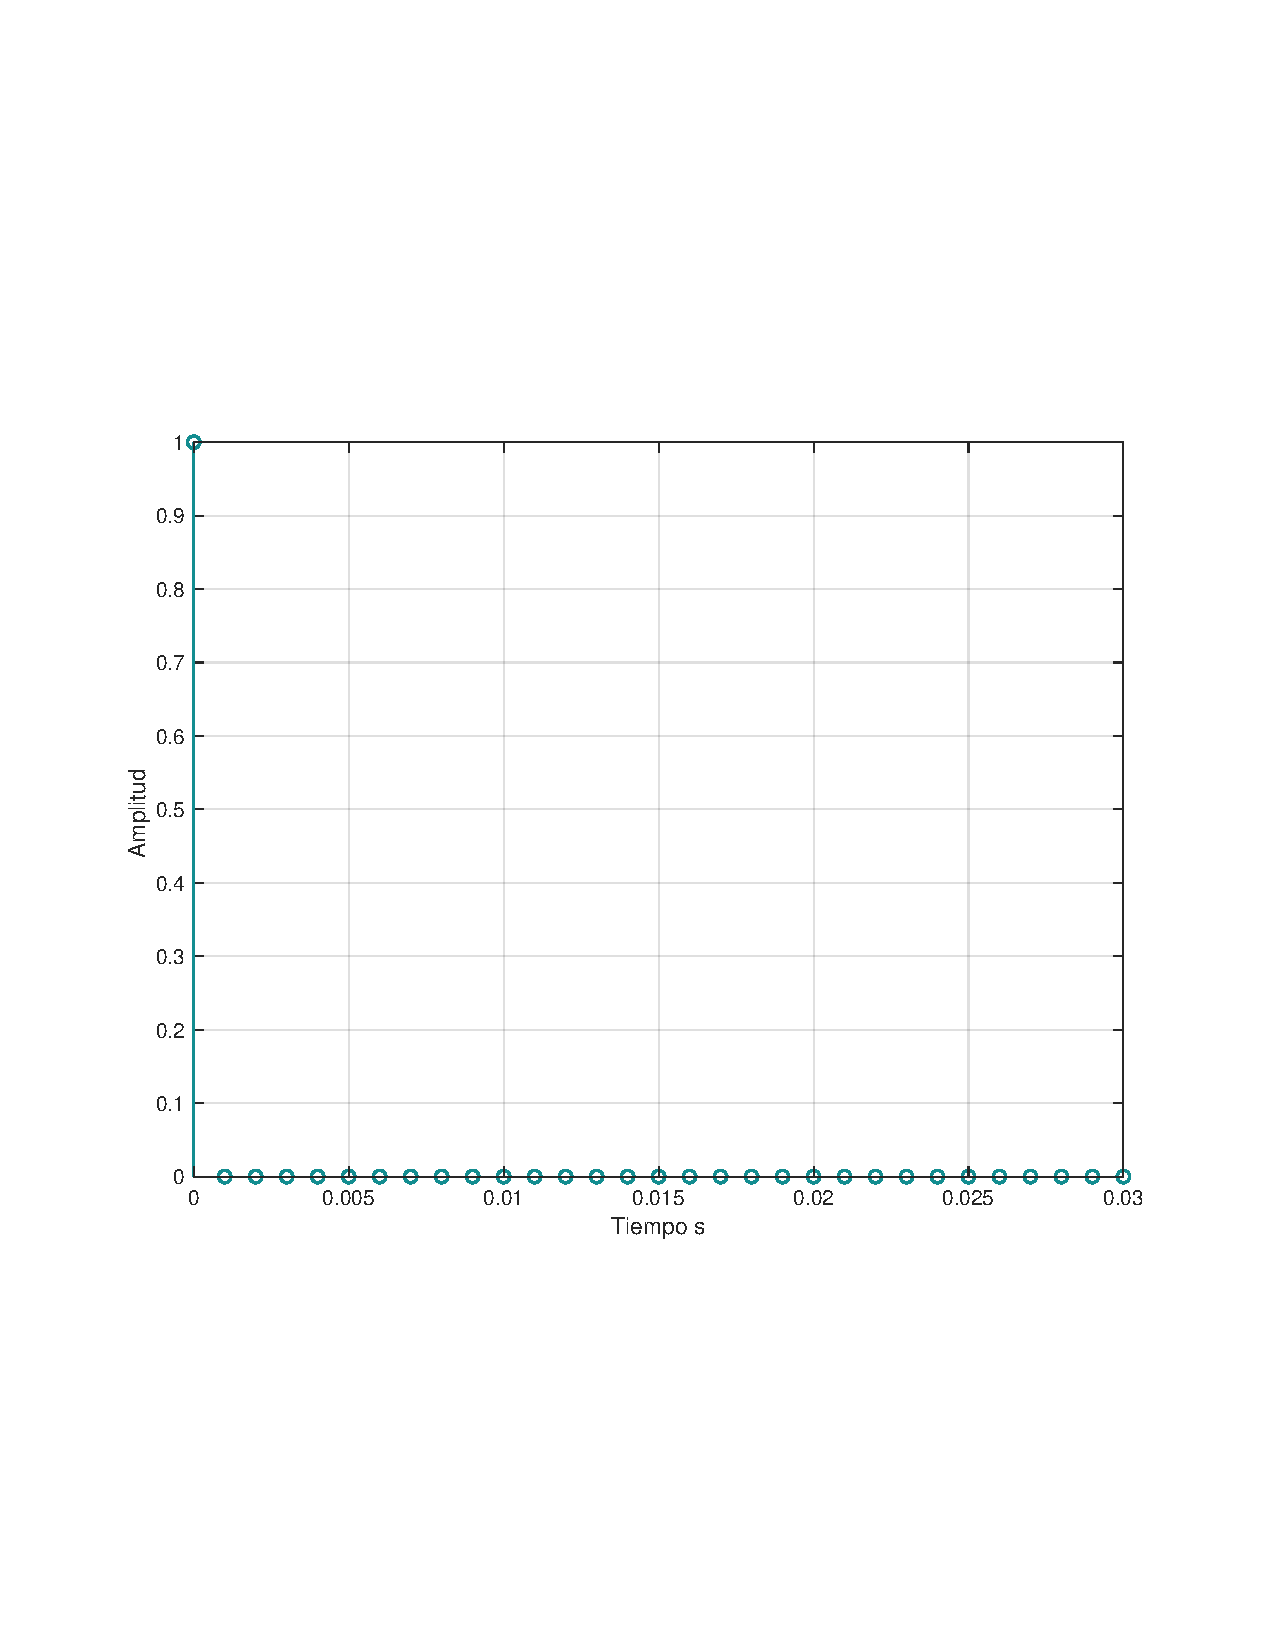
\includegraphics[width=0.6\textwidth,clip, trim = {2cm 7.0cm 2.2cm 7.0cm}]{../imgs/2_SbSa.pdf}
				\caption{Respuesta del sistema $S_{b}(S_{a}(x))$ a impulso}
 				\label{fig:2_SbSa}
 			\end{figure}
 			
 			Como se esperaba, dado que las funciones de transferencia son complementarias, el resultado es la misma señal de entrada.
 			
\section{Integrales y derivadas en tiempo discreto}
	Se considera, para tiempo continuo:
	\begin{align}
		y = S_{1}(x) \text{tal que } y(t) = \frac{d}{dt}x(t) \\
		y = S_{2}(x) \text{tal que } y(t) = \int_{-\infty}^{t} x(\tau)d\tau
	\end{align}
	
	\subsection{Aproximaciones de tiempo discreto}
		\subsubsection{Derivada}
			Consideremos la definición formal de la derivada temporal
			\begin{equation}
				\frac{d}{dt}x(t) = \lim_{h \rightarrow 0} \frac{x(t + h) + x(t)}{h}
				\label{eq:derivative_def} 
			\end{equation}
			
			Podemos realizar un análogo casi directo para tiempo continuo, considerando que la muestra $n-1$ y la muestra $n$, están separadas temporalmente por $T_{s}$. Expresando esto:
			\begin{equation}
				\frac{\Delta x[n]}{\Delta t} = \frac{x[n] - x[n-1]}{T_{s}} \approx \frac{d}{dt}x(t) |_{t = n}
			\end{equation}
			
			Llevando la expresión hallada a una forma de sistema:
			\begin{equation}
				\boxed{y[n] = \frac{x[n] - x[n-1]}{T_{s}}}
				\label{eq:derivative_S1}
			\end{equation}
			
			Analizando esta expresión, notemos que mientras la señal x[n] sea acotada y no presente \textit{saltos}, la salida y[n] será acotada, por lo que el sistema es \textbf{BIBO estable}. Notemos que esta aproximación de la derivada no es única, por ejemplo, se podría haber calculado como la diferencia entre la muestra n+1 y la muestra n, llegando al mismo resultado.
			
		\subsubsection{Integral}
			Considerando la definición por sumas de Riemann, de la integral:
			\begin{equation}
				\int_{a}^{b} f(x)dx =  \lim_{\Delta_{i} \rightarrow 0} \sum_{i = 1}^{n} f(t_{i}) \Delta_{i}
			\end{equation}			 
			
			Descomponiendo el término de la sumatoria, lo que obtenemos es que la suma del rectángulo de base $\Delta_{i}$ y altura $f(t_{i})$, con los rectángulos que le precedieron. Considerando que $\Delta_{i} = T_{s}$, podemos expresar esta idea en términos de ecuaciones de diferencia:
			\begin{equation}
				\boxed{y[n] = y[n-1] + T_{s}x[n]}
			\end{equation}
			
			La salida, está definida por el valor anterior de la salida y el área formada por el rectángulo de base $T_{s}$ y altura x[n]. Podemos saber que este sistema \textbf{no es BIBO estable}, considerando el caso donde se ingresa un escalón unitario a un integrador, ésta señal es acotada, pero si tendemos $t \rightarrow \infty$, el área bajo la curva, tenderá a ser infinita. 
			
	\subsection{Análisis con señal sinusoidal}
		Se considera una frecuencia de muestreo $f_{s} = 10$ \textit{KHz}. Consideramos una señal de prueba de las siguientes características:
		\begin{equation}
			x(t) =  \sin(2\pi\cdot 100 t)
		\end{equation}
		
		\begin{figure}[H]
			\center
			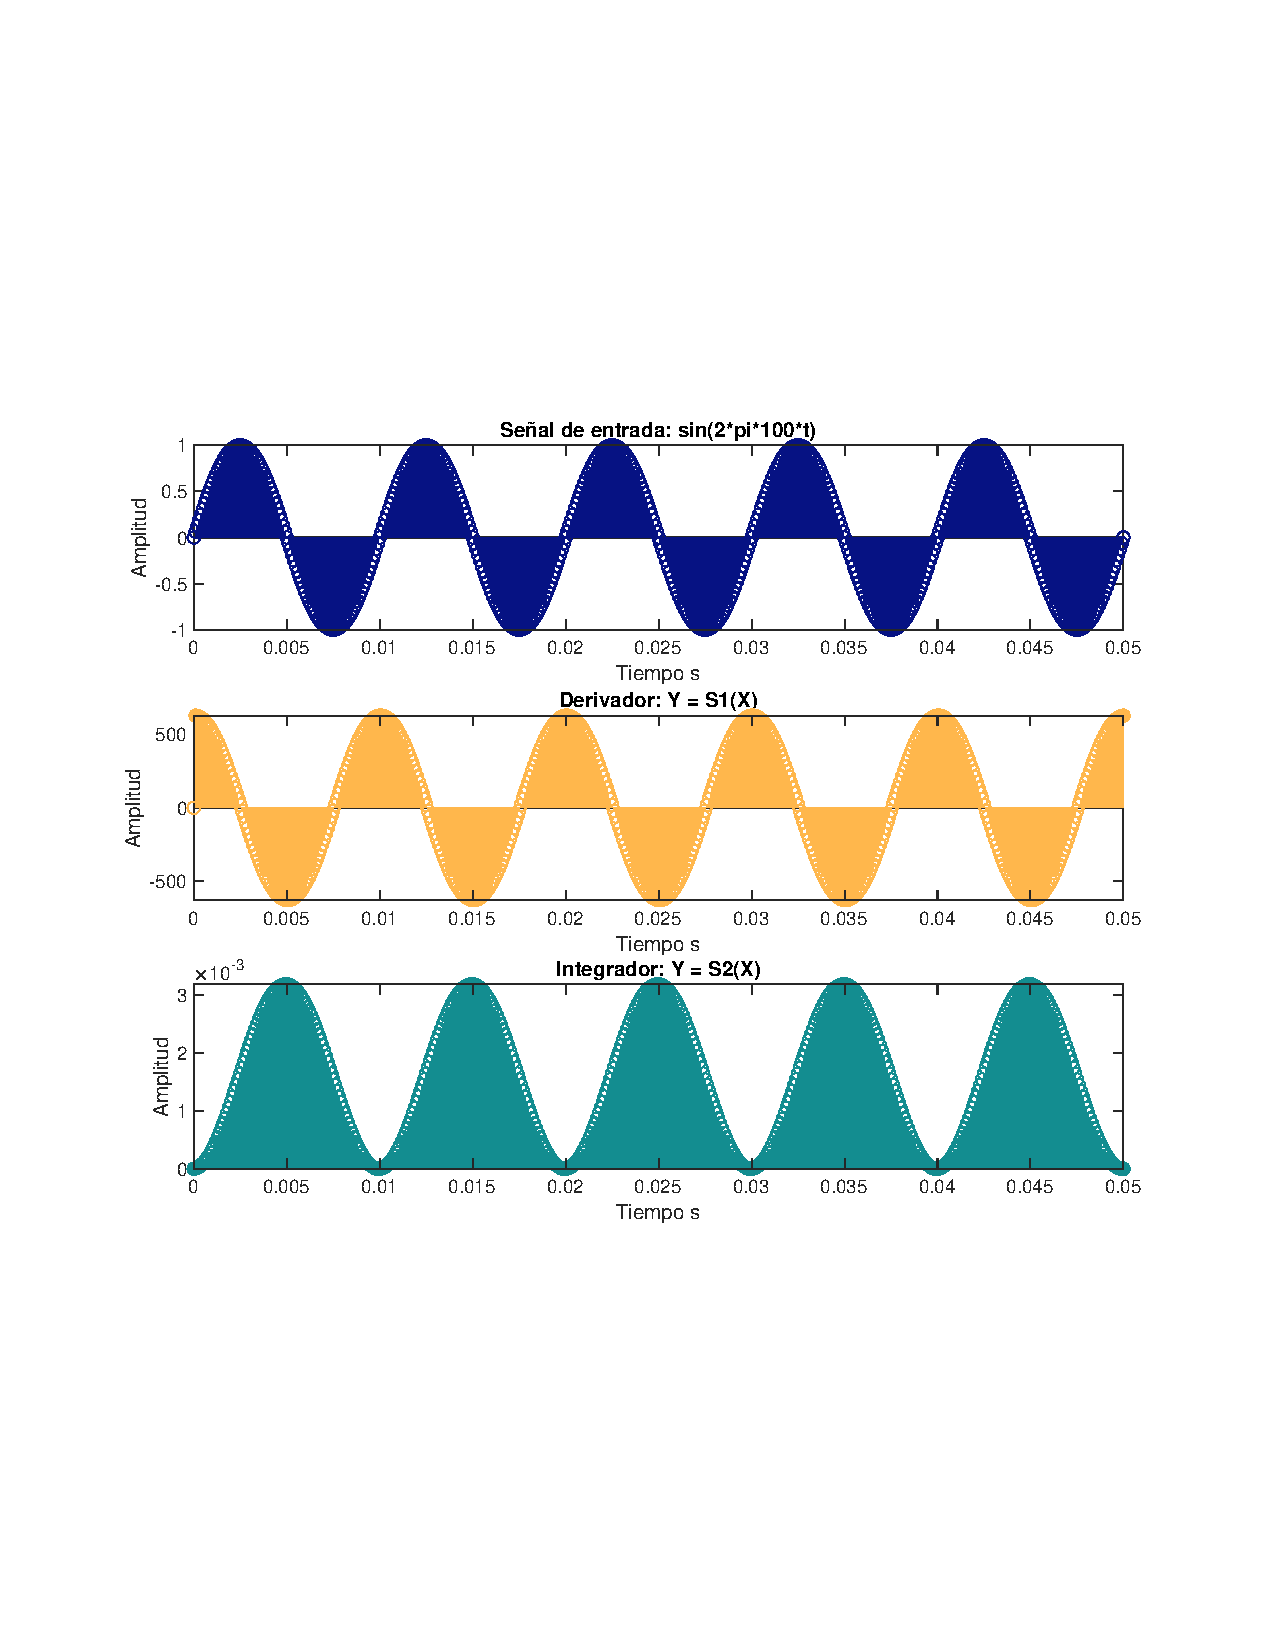
\includegraphics[width=0.6\textwidth,clip, trim = {2cm 7.0cm 2.2cm 7.0cm}]{../imgs/3_b.pdf}
			\caption{Resultado para la señal de entrada, en términos de su derivada e integral}
			\label{fig:3_b}
		\end{figure}
		
		Para el caso de la derivada, calculamos el valor esperado de manera teórica:
		\begin{equation}
			\frac{d}{dt}x(t) = 200\pi \cdot cos(200\pi t)
		\end{equation}
		
		Observando el resultado gráfico, notamos que la señal obtenida a la salida de S1(x), está desfasada en $\pi/2$ con respecto a la señal original, lo que nos permite concluir que es un coseno. Analizando la amplitud, se puede estimar que está acotada en un valor $|627| \approx 200\pi$ lo que corresponde con la expresión teórica para la derivada de un seno. 
		
		Para el caso de la integral, el valor esperado de manera teórica:
		\begin{equation}
			\int sin(200\pi t) dt = \frac{-1}{200\pi} cos(200\pi t) + C
		\end{equation}
		
		Considerando que el valor inicial en t = 0, será cero:
		\begin{align}
			C = \frac{1}{200\pi} \\
			\therefore \int sin(200\pi t) dt = \frac{-1}{200\pi} cos(200\pi t) + \frac{1}{200 \pi}
		\end{align}
		
		Notamos que el resultado gráfico, corresponde a lo esperado, dado que a medida que la señal avanzan en un período, el área bajo la curva, incrementa hasta alcanzar un máximo, para luego retornar a cero al cumplirse un período. El valor máximo que alcanza el área es $0.032$, que corresponde al caso donde se cumple medio periodo de la señal, valor que corresponde a lo esperado de manera teórica. 
	\subsection{Derivada e integral de: composicion de deltas}
		Se define la señal de entrada como:
		\begin{equation}
			x[n] = \delta [n] - \delta [n-5] 
		\end{equation}
		
		\begin{figure}[H]
			\center
			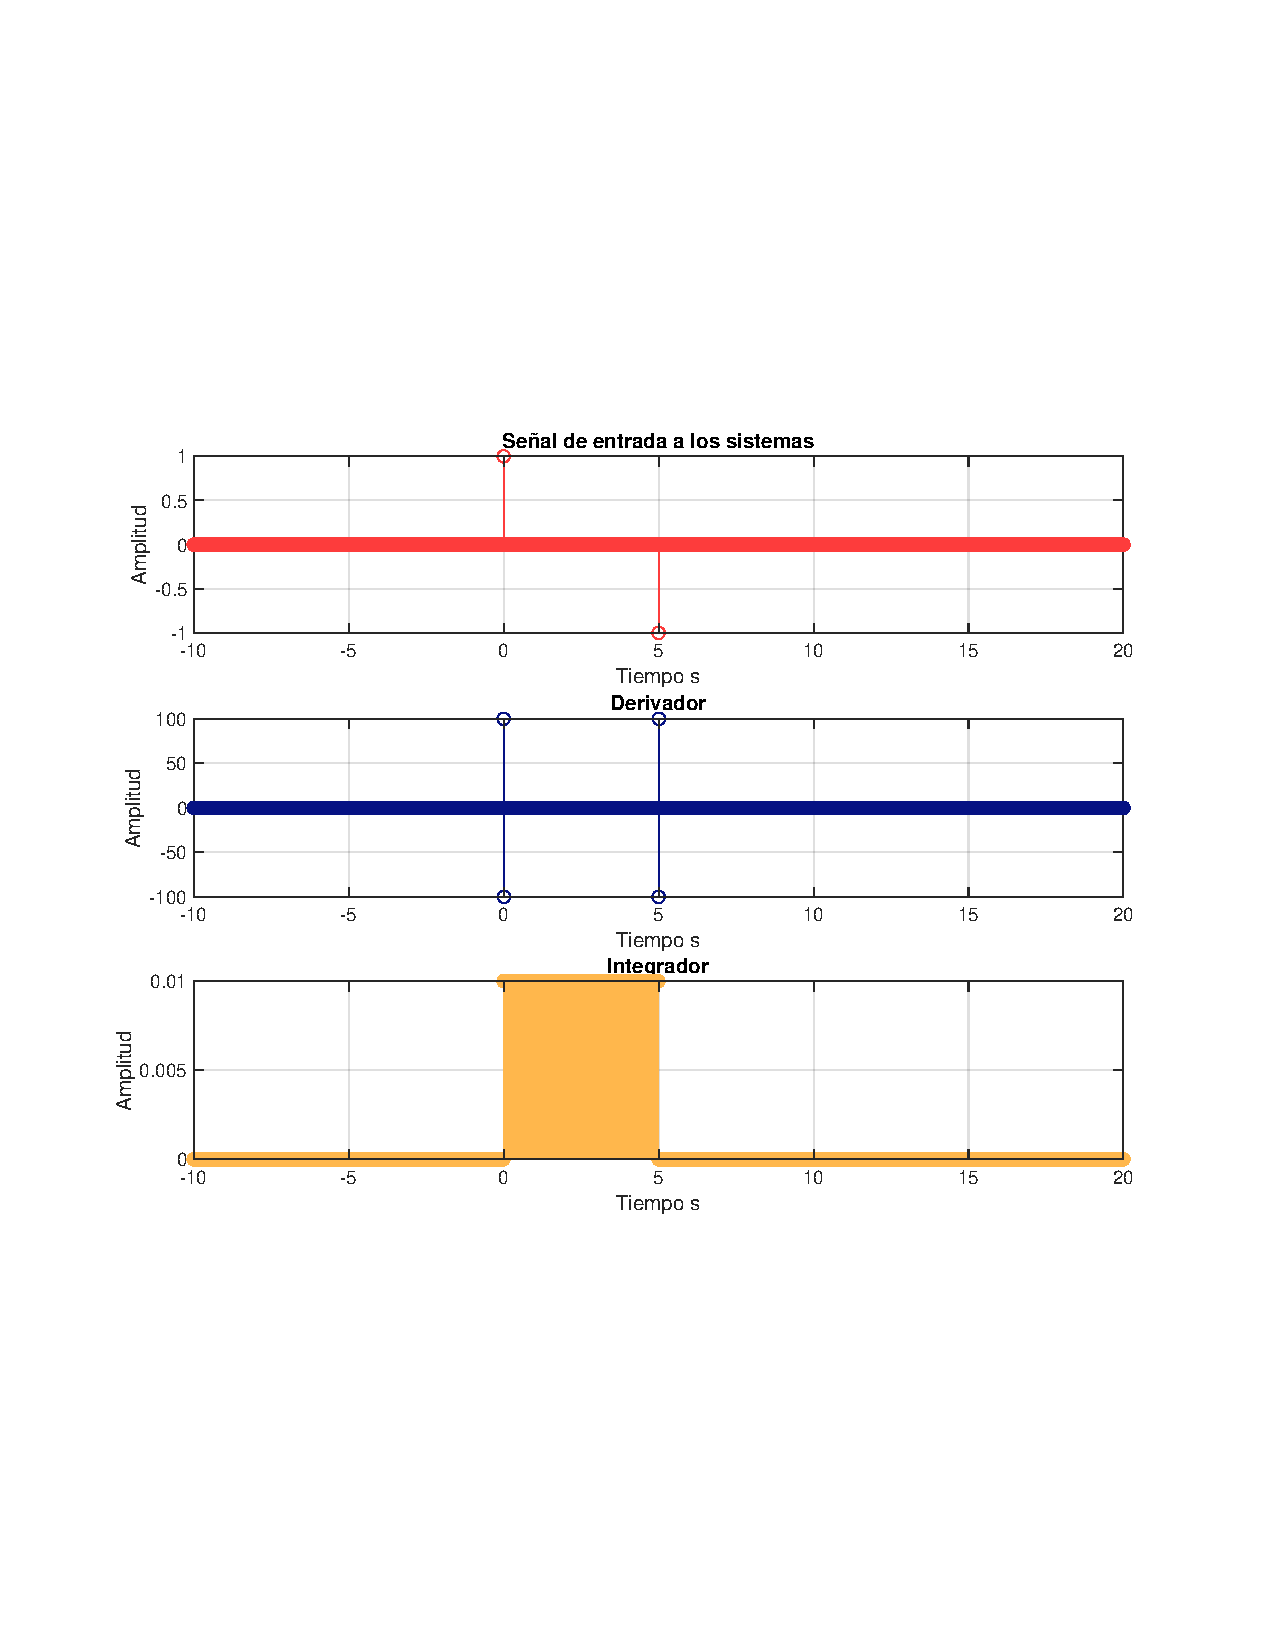
\includegraphics[width=0.6\textwidth,clip, trim = {2cm 7.0cm 2.2cm 7.0cm}]{../imgs/3_c.pdf}
			\caption{Resultado para la señal de entrada, en términos de su derivada e integral}
			\label{fig:3_c}
		\end{figure}
		
		Analizando los resultados, notemos que son coherentes a lo que se obtendría de manera teórica. Para el caso de la derivada, consideremos lo que pasa cuando nos acercamos al delta, estamos en valores de la señal de entrada que son cero. Cuando se llega al delta, la derivada se definira como la diferencia entre un valor muy alto y un valor cero, el cual será positivo, lo que da como salida un delta con valor positivo. A medida que nos alejamos del delta, esta diferencia ahora será entre un valor cercano a cero y un valor muy grande, lo cual arrojara un delta negativo. En el caso de la integral, es conocido que la integral de un delta corresponde a un escalón unitario.
	\subsection{Derivada e integral de: composición de escalones unitarios}
		 Se define la señal de entrada como:
		\begin{equation}
			x[n] = \mu [n] - \mu [n-5] 
		\end{equation}
		
		\begin{figure}[H]
			\center
			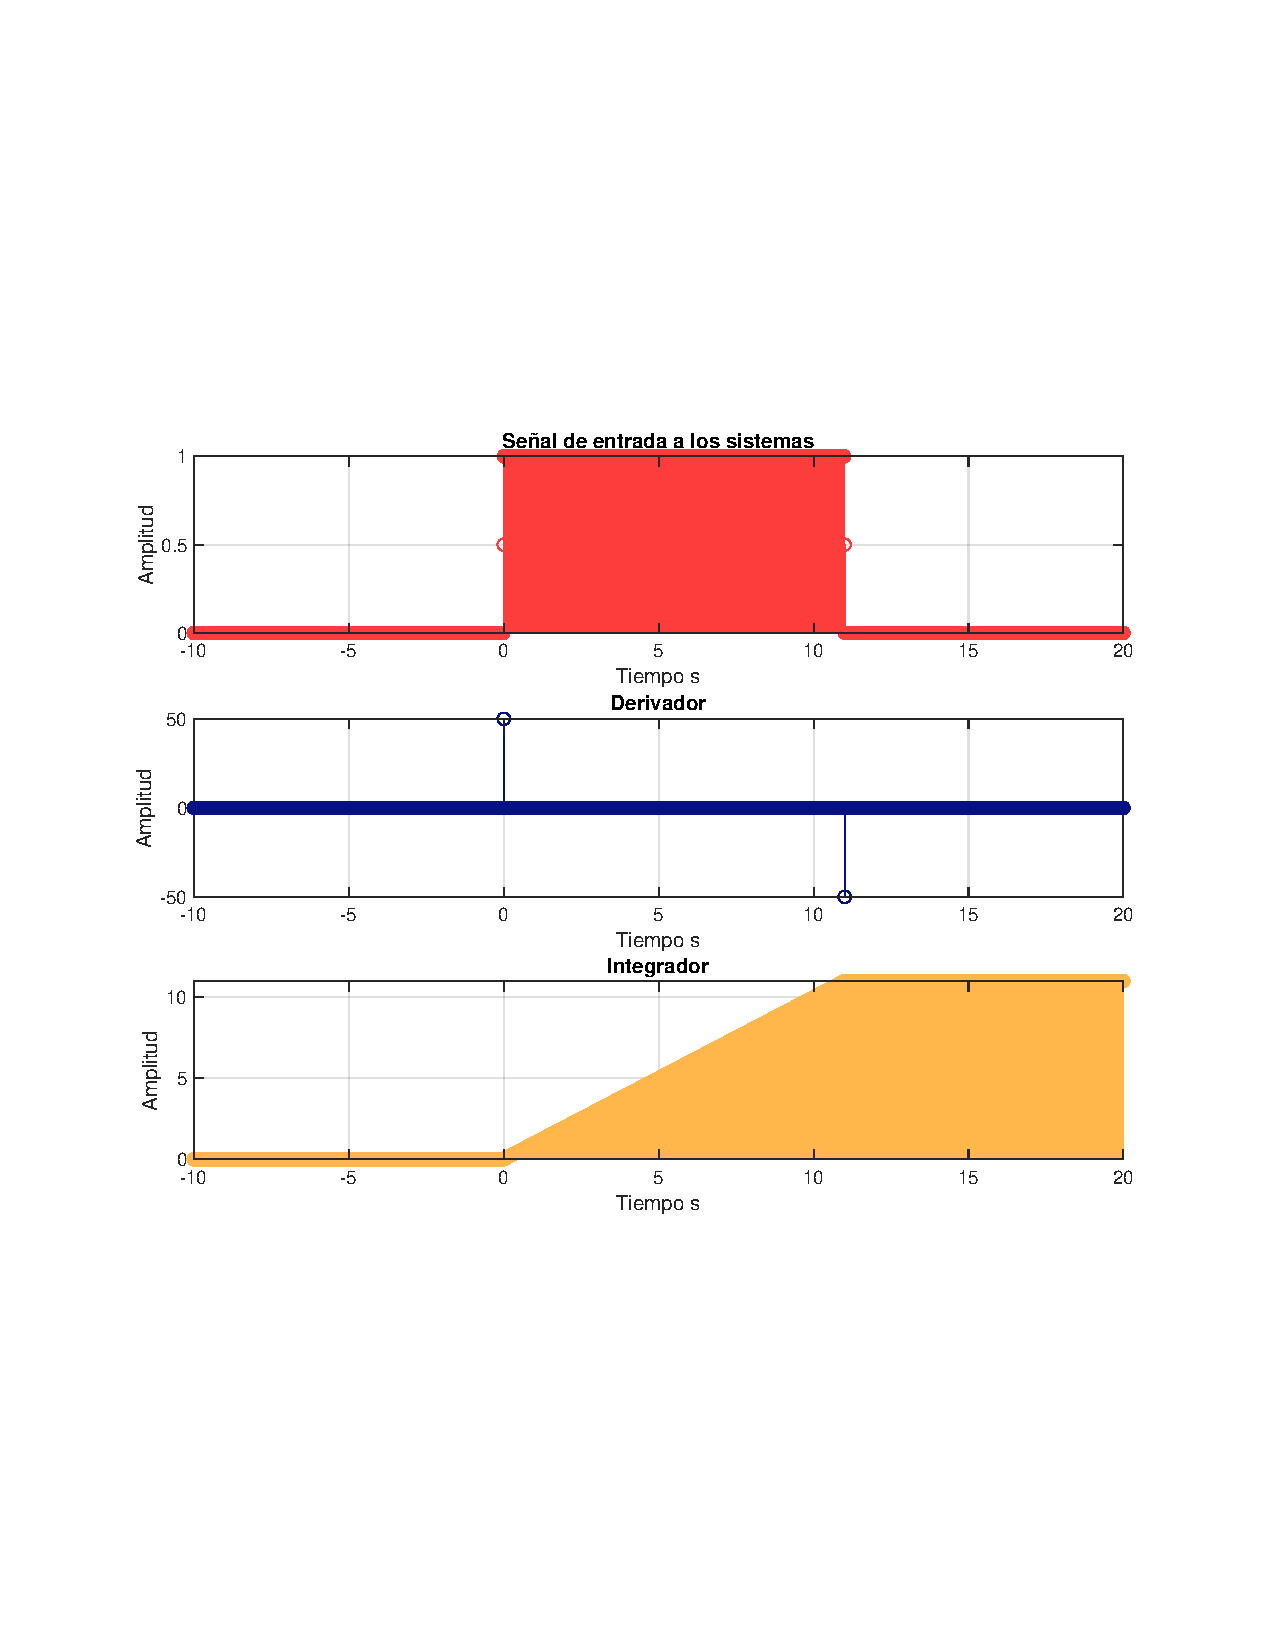
\includegraphics[width=0.6\textwidth,clip, trim = {2cm 7.0cm 2.2cm 7.0cm}]{../imgs/3_d.pdf}
			\caption{Resultado para la señal de entrada, en términos de su derivada e integral}
			\label{fig:3_d}
		\end{figure}
		
		Nuevamente el resultado es lo esperado, al derivar la composición de escalones, se obtendrá por definición dos deltas. En el caso de la integración, se obtendrá una señal que aumenta en amplitud junto con el área, hasta que se activa el segundo escalón que hace que el área se vuelva constante, por lo tanto la salida también. 
		
	\subsection{Derivada e integral de señales de audio}
		\subsubsection{Derivada}
			Al pasar la señales por el sistema de derivación, se siente que sólo quedan las componentes de alta frecuencia al escuchar la señal. Esto se debe a que la derivada actua como un filtro pasa altos, las componentes de menos frecuencia son atenuadas mientras que las señales con componentes de frecuencia altas pasan sin ser afectadas.
		\subsubsection{Integral}
			Este sistema se comporta de manera inversa al anterior, la integral actúa como un filtro pasabajos, componentes espectrales de baja frecuencia tienen un mayor efecto que componentes de frecuencia más alta, por esto al escuchar la señal esta se siente más apagada. 

	\subsection{Doble derivada y doble integral}
			Para poder determinar estos sistemas es conveniente expresar $S_{1}$ y $S_{2}$ mediante su función de transferencia en el dominio Zeta:
			\begin{align}
				H_{1}[z] = f_{s}\frac{z-1}{z} \\
				H_{2}[z] = \frac{1}{fs} \frac{z}{z-1} 
			\end{align}
			
			Se puede considerar cada una de estas funciones como un filtro, por lo que para conseguir la segunda derivada o integral, basta con poner los filtros en cascada.
			\subsubsection{Doble derivada S1(S1(x))}
				\begin{equation}
					\frac{d}{dt}x(t)|_{n} \approx h_{1}[n] * h_{1}[n]
				\end{equation}
				
				En el dominio de la transformada zeta:
				\begin{equation}
					H_{11}[z] = f_{s}^{2} \frac{z^{2} -2z + 1}{z^{2}}
				\end{equation}
				
				Como ecuación de diferencias:
				\begin{equation}
					y[n] = \left( x[n] - 2x[n-1] + x[n-2] \right) f_{s}^{2}
				\end{equation}
				
				Para este caso,  se tiene que mientras la señal de entrada sea acotada, la salida también lo será, por lo que el sistema es \textbf{BIBO estable}. El sistema se comporta como un filtro pasa-altos.
				
			\subsubsection{Doble derivada S2(S2(x))}
				\begin{equation}
					\int_{-\infty}^{t}\int_{-\infty}^{r}x(\tau)d\tau \approx h_{2}[n] * h_{2}[n]
				\end{equation}
				
				En el dominio de la transformada zeta:
				\begin{equation}
					H_{22}[z] = \frac{1}{f_{s}^{2}} \frac{z^{2}}{z^{2} -2z + 1}
				\end{equation}
				
				Como ecuación de diferencias:
				\begin{equation}
					y[n] = \frac{1}{f_{s}^{2}} x[n] + 2y[n-1] - y[n-2]
				\end{equation}
				
				Como se demostró anteriormente la integral es un sistema inestable, por lo que la doble integral también es \textbf{inestable}. Este sistema se comporta como un filtro pasabajos. 
				
			\subsubsection{Derivada de una integral e integral de una derivada}
				Note que ambos sistemas son análogos, sabiendo que son operaciones recíprocas (sus funciones de transferencia son recíprocas), el efecto de poner cualquier permutación de estos filtros será la misma:
				\begin{equation}
				H_{1}[z] \cdot H_{2}[z] = H_{2}[z] \cdot H_{1}[z] = 1 
				\end{equation}
				
				El sistema se comporta de manera transparente, la entrada es igual a la salida. La estabilidad estará dada únicamente por la estabilidad de la entrada.